% This is the root file of the thesis: thesis.tex

%%===================================
% \documentclass[12pt, oneside]{report}
\documentclass[12pt, twoside]{report}

\usepackage{url}
\usepackage[utf8]{inputenc} % This defines the font-encoding you prefer to use
\usepackage[pdftex]{graphicx}
\usepackage[bindingoffset=1cm,centering,includeheadfoot,margin=2cm]{geometry}

\usepackage[
    citestyle=numeric-comp,
    backend=biber,
    bibencoding=inputenc
    ]{biblatex}
\addbibresource{refs.bib}

\usepackage{setspace}
\linespread{1.5}
\setcounter{tocdepth}{2} 
\usepackage[colorlinks=true, pdfstartview=FitV,
linkcolor=blue, citecolor=blue, urlcolor=blue]{hyperref}
\setlength{\parindent}{0pt} % No indentation between paragraphs
\setlength{\parskip}{10pt} % Space between paragraphs

% Tables
\usepackage{ltxtable}
%\usepackage{arydshln}
%\usepackage{tabu, longtable}
\usepackage{booktabs}

% Needed for code listings
\usepackage{listings}
\usepackage{color}

% Subfigure
\usepackage{subcaption}

\usepackage{floatpag} % to move floatpagenr to topright

% Fussnote
\usepackage[hang]{footmisc}
\setlength{\footnotemargin}{-0.8em}

\usepackage{csquotes}
\usepackage{afterpage} % needed for empty page after front

%%===================================
% Custom definitions
    
% Signal color
\definecolor{signalColor}{RGB}{164, 63, 114}
\newcommand\signal[1]{\textbf{\textcolor{signalColor}{#1}}}
    
% List with less space between items
\newenvironment{cList}{
\begin{itemize}
  \setlength{\itemsep}{0pt}
  \setlength{\parskip}{0pt}
  \setlength{\parsep}{0pt}
}{\end{itemize}}

% Enumeration with less space between items
\newenvironment{cEnum}{
\begin{enumerate}
  \setlength{\itemsep}{0pt}
  \setlength{\parskip}{0pt}
  \setlength{\parsep}{0pt}
}{\end{enumerate}}

% Space LoL
\let\Chapter\chapter
\def\chapter{\addtocontents{lol}{\protect\addvspace{10pt}}\Chapter}

% Code definition JSON
\definecolor{numberColor}{RGB}{24,118,129}
\newcommand\JSONnumbervaluestyle{\color{numberColor}}
\newcommand\JSONstringvaluestyle{\color{signalColor}}

\newif\ifcolonfoundonthisline

\makeatletter

\lstdefinestyle{json}{
  showstringspaces    = false,
  keywords            = {false,true},
  alsoletter          = 0123456789.,
  morestring          = [s]{"}{"},
  stringstyle         = \ifcolonfoundonthisline\JSONstringvaluestyle\fi,
  MoreSelectCharTable =%
    \lst@DefSaveDef{`:}\colon@json{\processColon@json},
  basicstyle          = \ttfamily,
  keywordstyle        = \ttfamily\bfseries
}

\lstset{
  numbers=left,
  lineskip={-1.5pt},
  captionpos=b,
  basicstyle=\footnotesize\ttfamily,
  xleftmargin=1cm,
  breaklines=true
}

\newcommand\processColon@json{%
  \colon@json%
  \ifnum\lst@mode=\lst@Pmode%
    \global\colonfoundonthislinetrue%
  \fi
}

\lst@AddToHook{Output}{%
  \ifcolonfoundonthisline%
    \ifnum\lst@mode=\lst@Pmode%
      \def\lst@thestyle{\JSONnumbervaluestyle}%
    \fi
  \fi
  \lsthk@DetectKeywords% 
}

\lst@AddToHook{EOL}%
  {\global\colonfoundonthislinefalse}

\makeatother
% End code definition JSON

% Rename listings and toc
\renewcommand{\contentsname}{Table of Contents}
\renewcommand{\lstlistlistingname}{List of Listings}

\begin{document}

%%========================================
% Frontmatter

%!TEX root = ../thesis.tex

%This is the front page
%%=========================================
\thispagestyle{empty}


\includegraphics[width=\linewidth]{fig/Logo_Header}
\mbox{}\\[1pc]
\begin{center}
    \huge{ \bfseries Using Reinforcement Learning to Size Tasks for Scientific Workflows}\\[2pc]

    \Large{Nicolas Zunker}\\
    \large{n.zunker@campus.tu-berlin.de}\\[1pc]
    \large{December 13, 2021}\\[2pc]

    BACHELOR'S THESIS\\
    Distributed and Operating Systems Chair\\
    Technische Universität Berlin
\end{center}
\vfill

Examiner 1: Prof. Dr. Odej Kao
\hfill\llap{Advisor: Jonathan Bader}\\
Examiner 2: Prof. Dr. Volker Markl

\afterpage{\null\thispagestyle{empty}\newpage}
 % This is the titlepage
\setcounter{page}{0}
\pagenumbering{Roman}
%!TEX root = ../thesis.tex

%This is the Preface
%%=========================================
\cleardoublepage
\section*{Declaration}
\addcontentsline{toc}{section}{Declaration}
I hereby declare that I have created the present work independently and by my own without illicit assistance and only utilizing the listed sources and tools.\\

Hiermit erklaare ich, dass ich die vorliegende Arbeit selbststaandig und eigenhaandig sowie ohne unerlaubte fremde Hilfe und ausschliesslich unter Verwendung der aufgefaehrten Quellen und Hilfsmittel angefertigt habe.

Die selbständige und eigenständige Anfertigung versichert an Eides statt:
\begin{center}
Berlin, den 13. Dezember 2021\\[3pc]
Nicolas Zunker
\end{center}

%!TEX root = ../thesis.tex

%This is the Acknowledgment
%%=========================================
\cleardoublepage
\addcontentsline{toc}{section}{Acknowledgment}
\section*{Acknowledgment}

I would like to thank my advisor Jonathan for his helpful advice, constructive feedback and assistance, Prof. Dr. Toussaint, Prof. Dr. habil. Kao and Prof. Dr. Zubow whose courses I enjoyed immensely and from whom I learned a lot, and my friends and family for their support.

\nocite{fan2020,learningToSchedule,scarl,toussaint}


\begin{flushright}
NZ\\[1pc]
\end{flushright}

%!TEX root = ../thesis.tex

%This is the Summary
%%=========================================
\cleardoublepage
\addcontentsline{toc}{section}{Abstract}
\section*{Abstract}

The growth of computational power and the increasing importance of digital data in scientific research has led to greater demand for computational resources  by users who aim to process large datasets. Particularly in the natural sciences it has become common for scientists to break down their computing needs into a sequence of smaller tasks, a so called workflow. These workflows can then be run on a variety of different execution platforms, depending on the users needs.

Since workflows are composed of segregated inter-dependent tasks which can run independently of each other, the individual tasks which make up a workflow can be assigned a fraction of the computational resources available to the entire execution platform, and doing so intelligently could improve efficiency and performance.

This thesis aims to investigate how reinforcement learning can be applied to the allocation of resources to individual tasks in order to choose more efficient allocations. A reinforcement learning solution will be integrated into the source code of a popular scientific workflow management system and tested with several common bioinformatic workflows. Two different approaches (Gradient Bandits and Q-learning) will be used and their performance will be compared with both that of the default resource allocations and that of an approach based on \cite{tovarjob,FeedbackBasedAllocation} which uses a feedback loop.

Ultimately the approaches presented in this thesis outperform the workflow's default configurations with regards to both memory and CPU efficiency: the q-learning approach assigned 7\% less CPU hours, 31\% less memory and was 7\% faster, whereas the gradient bandit approach assigned 42\% less CPU hours, 80\% less memory and was only 4\% slower. The feedback loop approach assigned 13\% less CPU hours, 87\% less memory and was 7\% faster and thus performed worse than the gradient bandits with regards to CPU efficiency but better in terms of memory and speed. 

%%=========================================
%\cleardoublepage
\addcontentsline{toc}{section}{Zusammenfassung}
\section*{Zusammenfassung}

Die Relevanz von digitalen Daten und die damit verbundene Analyse von grossen Datensätzen in der wissenschaftlichen Forschung wächst kontinuierlich, und der Nutzerbedarf an Rechenressourcen steigt mit. Besonders in den Naturwissenschaften ist es üblich, dass Wissenschaftler die Analyse dieser Daten in kleinere Arbeitspakete aufteilen, so genannten Tasks, und die gesamte Sequenz dieser Tasks wird als Workflow bezeichnet. Die Workflows bestehen aus verschiedenen, eigenständigen Tasks die unabhängig voneinander ausgeführt werden können, daher muss ihnen nur ein Bruchteil der Rechenressourcen des Plattforms auf dem sie ausgeführt werden zugewiesen werden.  Durch intelligente Allokationen ermöglicht dies eine größere Effizienz und Leistung der Workflows.  

Die Forschungsfrage dieser Arbeit beinhaltet wie und mit welchem Effekt Reinforcement Learning für die Allokation von Rechenressourcen zu den Tasks eines Workflows angewandt werden kann.  Hierzu werden zwei verschiedene Ansätze (Q-learning und Gradient Bandits) in den Quellcode einer Workflow Verwaltungssoftware integriert und mit fünf Bioinformatik Workflows getestet. Diese Ergebnisse werden verglichen mit der Leistung der Workflows unter normalen Konfigurationen, und einem Ansatz mit Hilfe von Rückkopplungsschleifen, der auf \cite{tovarjob,FeedbackBasedAllocation} basiert.

Die in dieser Arbeit entwickelten Ansätze zeigten eine bessere Leistung als die Workflows mit voreingestellten Allokationen, sowohl im Bezug auf die Arbeitsspeichernutzung, als auch auf die CPU Nutzung.  Der q-learning Ansatz allozierte 7\% weniger CPU Stunden, 31\% weniger Arbeitsspeicher und die Rechenleistung war 7\% schneller. Der gradient bandit Ansatz allozierte 42\% weniger CPU Stunden, 80\% weniger Arbeitsspeicher und die Rechenleistung war nur 4\% langsamer. Letztlich hat der Ansatz mit der Rückkopplungsschleife 13\% weniger CPU Stunden und 87\% weniger Arbeitsspeicher alloziert und war 7\% schneller, und damit weniger effizient mit seiner CPU Allokationen als die gradient bandits aber besser in Bezug auf Arbeitsspeicher und Geschwindigkeit.

%\newpage
%\addcontentsline{toc}{section}{Zusammenfassung}
%\section*{Zusammenfassung}

%Der Aufstieg des Internet of Things (IoT) stellt uns vor neue Herausforderungen bezueglich der Speicherung, Verarbeitung und Darstellung von Daten

\tableofcontents

\clearpage
\phantomsection
\addcontentsline{toc}{section}{\listfigurename}
\listoffigures

\clearpage
\phantomsection
\addcontentsline{toc}{section}{\listtablename}
\listoftables

\clearpage
\phantomsection
\addcontentsline{toc}{section}{\lstlistlistingname}
\lstlistoflistings

%%=========================================
% Mainmatter

\cleardoublepage
\setcounter{page}{0}
\pagenumbering{arabic}
%!TEX root = ../thesis.tex

\cleardoublepage
\chapter{Deterministic Multipath Backhaul Exposee - Masters Thesis}

\label{cha:introduction}

%%=========================================
\section{Motivation and Problem Description}
\label{sec:motivation}

One of the aims for the fifth generation of mobile networks (5G) and it's successors will be a greater diversification of the classes of service. As the use cases for these networks evolve, there is a greater need for quality of service (QoS) tailored to each use case. For example, in Industrial Internet of Things (IIoT) applications the bandwidth requirements are often quite low, however the requirements on latency, jitter, and reliability may be extremely stringent. Supporting these kinds of classes of service can be a challenge for mobile network operators (MNOs) and will require novel approaches to familiar problems, such as backhaul.

With more backhaul solutions becoming available (i.e. LEO satellite links, and mmWave backhaul) and adding to the existing set of options (DSL, optical fibre, DOCSIS, dedicated lines, etc.) network operators may choose to utilize more than one backhaul connection at once in order to increase the available bandwidth or to utilize the different qualities of the backhaul links. Such a situation, could then be used to achieve higher quality of service by intelligently selecting on which link to forward packets. This approach bears similarity to multihoming as well as to multi-path routing, and can take inspiration from the existing body of research in these fields which has demonstrated that QoS can be improved by using multiple paths simultaneously \cite{akella2003measurement, tao2005improving, habib2007improving, goldenberg2004optimizing, huang2008multiconstrained, akella2008performance}.


%\LTXtable{\textwidth}{tab/scenario1_sensor}

%%=========================================
\section{Goal of the Thesis}
\label{sec:goal}

\begin{figure}[h]
    \centering
        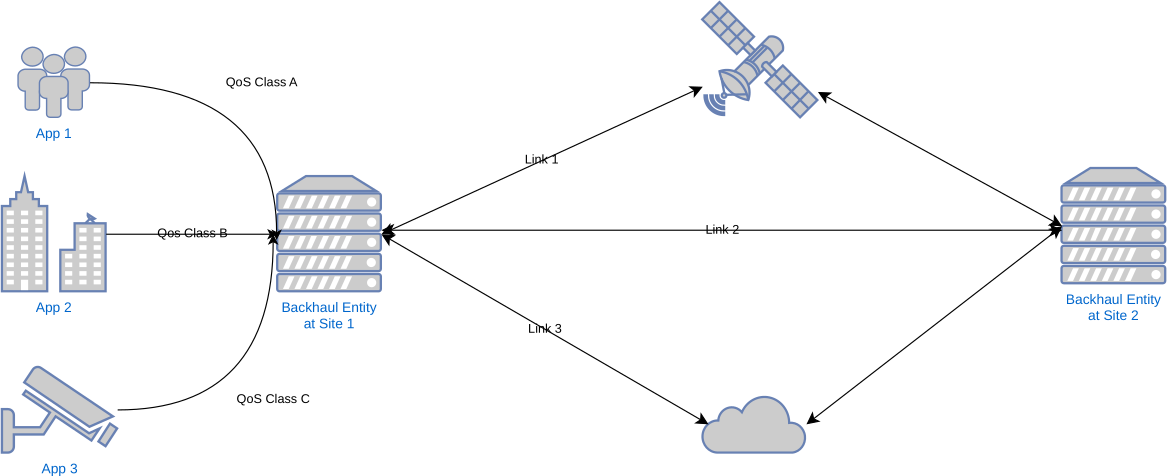
\includegraphics[width=\textwidth]{fig/use_cases.png}
        \caption{Use Case for the Backhaul Entity}
        \label{fig:use}
\end{figure}


\begin{figure}[h]
    \centering
        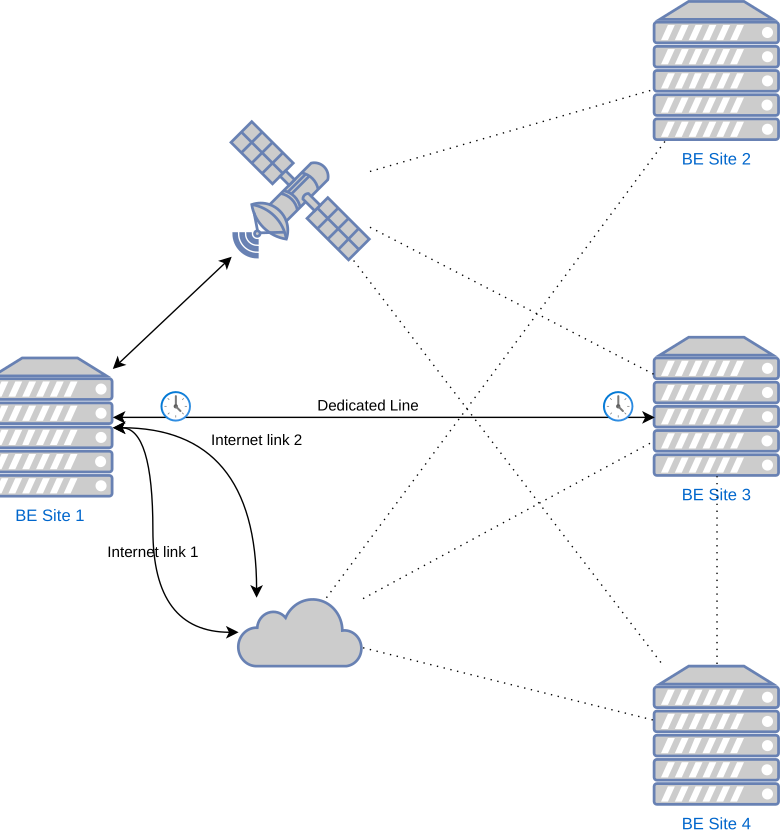
\includegraphics[width=0.75\textwidth, height=0.75\textwidth]{fig/mesh_network.png}
        \caption{Network of Backhaul Entities}
        \label{fig:mesh}
\end{figure}

The goal of this thesis is to design a backhaul entity, that can be placed at the ingress and egress point of connected networks, and which can intelligently forward packets on one or more links in order to meet specific QoS requirements. The performance of this approach will then be quantitatively analysed in experiments. Looking at figure \ref{fig:use} we can see how this is envisioned to work: A backhaul entity is deployed in 2 or more sites which have more than one egress link. Then, using the multiple links, the traffic is backhauled to the second site, while respecting it's QoS requirements. An example of how this entity could be deployed in multiple sites, interconnected in a mesh network, can be seen in figure \ref{fig:mesh}. This could allow network operators to provide more reliable quality of service for it's users, especially for important applications (e.g. between industrial sites).

%%=========================================
\section{Structure of the Thesis}
\label{sec:structure}

The planned work for the thesis will be structured as follows:

\begin{enumerate}
\item{\textit{Design}: Research existing approaches and solutions, and design an approach for reliable backhaul over multiple paths/links}
\item{\textit{Implementation}: Implement said approach in a basic testbed consisting of a traffic generator, various link emulators, measurement devices, and the backhaul entities}
\item{\textit{Evaluation}: Analyse the performance of the backhaul entity according to its ability to reduce latency, improve jitter, and provide any other QoS requirements. And compare it's performance with the performance of each individual link, as well as the performance of a round robin packet forwarding approach which utilises each link equally.}

\end{enumerate}

\begin{figure}[h]
    \centering
        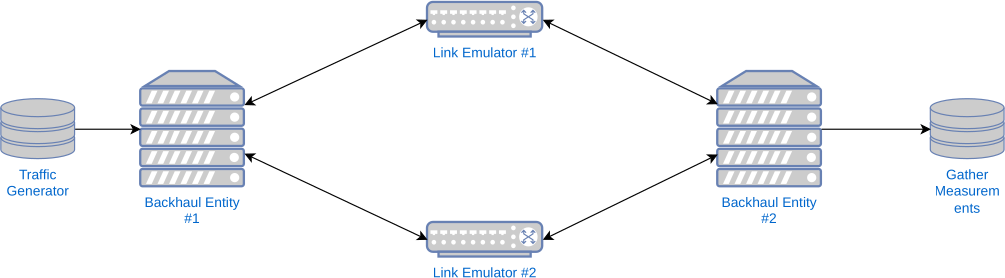
\includegraphics[width=\textwidth]{fig/testbed.png}
        \caption{Testbed Setup}
        \label{fig:testbed}
\end{figure}

The structure of the report will be a simple 5 chapter format: 1) Introduction, 2) Background and Related Work, 3) Approach, 4) Evaluation, 5) Conclusion. The approach chapter will discuss the proposed solution, and the evaluation chapter will encompass the design of the testbed and an analysis of the results.

\subsection{Timescale}

A thesis should take 6 months, or roughly 26 weeks. At present it is proposed to divide those 26 weeks into 4 equal sized chunks. The first 3 chunks will correspond to the 3 items mentioned previously in this section, the final "chunk" will be to finish writing up the report, however it is planned to do some writing during the other 3 chunks as well. In the first period - the \textit{Design} period, chapters 1 and 2 will also be worked on. After the \textit{Implementation} period is finished, chapter 3 can be written. Chapters 4 and 5 can then be written after the \textit{Evaluation} period finishes. That leaves the final chunk of time, which can be used to revise the document, as well as a buffer in case other parts of the thesis take longer to do.

The first phase of the experimental work will consist of setting up the testbed. This means installing the measurement modules as well as the link emulators. The next phase will require the implementation of the backhaul entity, as designed. The backhaul entity will require a module for collecting per-metric links, as well as the implementation of an algorithm to select the best link or links for a given flow. In the course of designing and preparing the backhaul entity there may be room for adjusting the initial plan based on what we experience during development. Next, the entity must be tested. During this phase traffic replays will be played over the testbed and evaluated. Thereafter the round robin approach and the "god routing" approach will also be evaluated. These two approaches will serve for comparison with the performance of the backhaul entity. Finally, this data must be analyzed, and the thesis can reach its conclusions, with 1 or 2 weeks buffer room for last minute revisions.


\begin{figure}
\begin{ganttchart}[expand chart=\textwidth, vgrid, hgrid]{1}{26}
  \gantttitle{Week}{26} \\
  \gantttitlelist{1,...,26}{1} \\
%  \ganttgroup{Group 1}{1}{7} \\
  \ganttbar{Literature Review}{1}{2}  \ganttbar[bar/.append style={fill=lightgray}]{}{3}{4} \\
  \ganttbar{Setup Testbed}{2}{4} \\
  \ganttbar{Implement Approach}{4}{8}] \ganttbar[bar/.append style={fill=lightgray}]{}{9}{10}  \\
  %ganttbar[bar/.append style={fill=lightgray}]{}{14}{14} \\
  \ganttbar{Metric Collection}{5}{7} \\
  \ganttbar{Link Switching Algorithm}{6}{8}\\
  \ganttbar{Adjust and Improve}{7}{9} \\
  \ganttbar{Measurements}{10}{16}  \ganttbar[bar/.append style={fill=lightgray}]{}{16}{18} \\
  \ganttbar{Round Robin}{12}{14} \\
  \ganttbar{God Routing}{14}{16}  \\
  \ganttbar{Evaluation}{18}{20}  \ganttbar[bar/.append style={fill=lightgray}]{}{21}{22} \\
  \ganttbar{Finish Writing Thesis}{21}{23}  \ganttbar[bar/.append style={fill=lightgray}]{}{24}{26} \\
  % \ganttlinkedbar{Task 2}{3}{7} \ganttnewline
 % \ganttmilestone{Milestone}{7} \ganttnewline
  \ganttlink{elem2}{elem3}
  \ganttlink{elem4}{elem8}
  \ganttlink{elem5}{elem8}  
  \ganttlink{elem6}{elem8}
  \ganttlink{elem7}{elem8}

 \ganttlink{elem9}{elem12}
 \ganttlink{elem10}{elem12}
 \ganttlink{elem11}{elem12}

\ganttlink{elem12}{elem14}

\end{ganttchart}
\caption{Gantt Chart: 01.06.23 - 01.12.23}
\end{figure}

\section{Envisioned Approach}

\subsection{Collecting Per-Link Metrics}

In order to realize such a backhaul entity, the entity needs to be able to maintain a set of metrics about the available links to aid it in choosing which links to utilize. This may not always be straightforward, and could require prediction of link quality based on previous measurements.

\subsubsection{Measurement-based Metrics}

In \cite{akella2008performance} the authors collected both passive metrics (looking at response times for outgoing packets), and active measurements (sending ICMP ping, or TCP SYN messages and measuring the response time). It is important to note that using the passive measurements enabled their multihomed approach to perform well, but when using the active measurements the performance was better. Crucially, the passive measurements worked better over larger sampling periods because it took longer to get a full overview of all the possible routes. Whereas the active sampling approach acquired it's measurements faster and was thus more effective over smaller sampling intervals.

Considering these results, it is proposed to utilize both active and passive measurements. All three metrics- packet loss, latency, and jitter- will be periodically measured in an active manner, on a site to site basis. The period over which to perform these measurements is an important design decision.

Beyond this, these metrics will also be monitored on a passive basis wherever possible. For all three metrics a response is required for each sent message, in order to measure either the time needed (for latency and jitter), or to ascertain a packet has been lost. This may only be possible for TCP SYN and SYN ACK messages, and other protocols which are guaranteed to contain certain request-response handshakes.

\subsection{Pre-configured Metrics}

Since certain links may be come with hard guarantees on packet loss, latency and jitter, this would drastically simplify the process, and thus allow us to save ourselves the measurement process for said links. Therefore the backhaul entity which will be designed, shall allow for a link to have the jitter, reliability and latency metrics pre-configured, as well as allowing them to be updated while the entity is running.

\subsection{How to Guarantee QoS}

The design of this approach is also an interesting challenge. One idea to improve jitter when backhauling across multiple links is to duplicate packets and forward them on multiple links, and have the backhaul entity on the other end buffer incoming packets and release them at a constant rate. This way in the event of a packet being lost on one link, the other link is still able to receive it and the delay caused by retransmission is avoided. The downside with this approach is that it guarantees the latency will always be that of the slowest link.

For reducing latency it would appear likely that the simplest approach may be a greedy method (as in \cite{goldenberg2004optimizing} in the online case) which always selects the lowest latency connection. However there is room for nuance here since the connection must not be overloaded and also because certain traffic may have very relaxed latency requirements but use up more bandwidth. This means monitoring the load on any one link will be important. Finally there are also more intelligent approaches, i.e. integer linear programming (used in \cite{huang2008multiconstrained} and for the offline case in \cite{goldenberg2004optimizing}) which could be used to optimally satisfy certain requirements.

The timescale over which to use a chosen link is also of interest. In \cite{habib2007improving} the time for which a link should be used is varied based on the predicted qualities of the link. These predictions are made based on past performance.

Reliability presents yet another challenge, however in a multihomed scenario it becomes easier to guarantee this via duplication, and/or forward error correction (FEC). For example if a packet flow requires 99\% reliability this can be guaranteed by duplicating packets across two links which are both only 90\% reliable. Alternatively, in such a situation, FEC could be used to pre-code the packets in order to provide the additional guarantees against packet loss and thus increase the reliability to the required level.

\subsubsection{Proposed Solution}

The solution proposed for solving this multi-constrained QoS problem is to use integer linear programming (ILP). Although ILP is NP-Complete, we can parameterize the problem by the number of outgoing links, which never needs to be more than 4, and thus brute force the solutions. The ILP constrained problem will be to select those links on which to forward packets while minimizing the overall number of links used, and making sure to satisfy the latency, jitter and reliability requirements of the given flow.

\begin{gather}
\text{Minimize } \sum_{i=1}^{P}x_i \\
\text{Where, } d(i) * x_i\le D \\
j(i) * x_i \le J \\
\text{and }1 - \prod_{i=1}^{P}{ ( 1- r(i) * x_i ) } \ge R  \\
\text{for } x_i \in \{0,1\}
\end{gather}

Here the variables $D$, $J$, and $R$ are the flow's delay, jitter, and reliability requirements, while the functions $d(i)$, $j(i)$, $r(i)$ are the predicted delay, jitter, and reliability of the link $i$ out of the $P$ total links. The predicted values will usually just be the latest measurement, as recommended in \cite{akella2008performance}, however there is room here to use more advanced metrics to predict the future link quality and thus perform preemptive path switching. The $x_i$ variable indicates whether or not link $i$ shall be used. If a solution is found, then the flow's packets will be forwarded on each link $i$ where $x_i = 1$, and if no solution can be found which satisfies these conditions then the flow is rejected because its QoS cannot be guaranteed.

\subsection{Potential Issues and Design Questions which are Still Open}

At present the idea would be to use the GTP protocol to tunnel data between any two backhaul entities, and then use the tunnel endpoint IDs (TEIDs) to differentiate between different traffic flows. In the control plane of the backhaul entity, one link would be chosen to be used for control and co-ordination messages between the two backhaul entities.

This approach could run into trouble if there is fragmentation. Some applications attempt to base their packet sizes on the most common MTU values for ethernet links (1500 bytes  minus 20 bytes for the IPv4 header and 2 bytes for UDP), and this causes a problem when the packet is tunneled because the overhead of another IP header on top of the tunnel header pushes the packet beyond the MTU and thus it has to be fragmented, which can degrade performance. In the proposed design of the testbed, there is a traffic generator at use, so this generator can be configured not to  generate packets exceeding 1450 bytes, but this issue is of practical concern for any realistic deployments.

\subsection{Evaluating Performance}

In order to evaluate the success of the proposed approach, three scenarios will be set up and investigated. Each setup will consist of two backhaul entities, and some number of emulated links going between them. The first scenario will feature 2 WAN links, a dedicated line, and a satellite connection. The second scenario will not feature the dedicated line, since it is expected that a leased line may be too obvious a choice for any of the traffic with strict QoS requirements. Finally, in order to further investigate these situations with an obviously superior candidate, the third scenario will just feature two links, a dedicated line and a WAN link.

In all of these scenarios the same traffic flows will be replayed. This traffic will contain various types of flows, with various QoS requirements. Before a new flow is started, the flow's requirements are sent to the backhaul entity and it is either accepted or rejected. During the traffic replay, the delay, jitter, and reliability will be measured.

These measurements will be performed once with the ILP approach proposed earlier and once with a simple round-robin approach for selecting links, and finally compared against an offline approach, where the optimal decision is computed with complete knowledge of the future. This offline approach will serve as the baseline for optimal performance, against which the other two approaches can be compared.


%%% include all citations

% start zotero

%\nocite{kundel_user_2022}
%\nocite{goldenberg_optimizing_nodate}
%\nocite{lange_performance_2015}
%\nocite{tarique_survey_2009}
%\nocite{tschoke_time-sensitive_2021}
%\nocite{ganichev_yamr_2010}
%\nocite{habib_improving_2007}
%\nocite{tao2005improving}
%\nocite{fanglu_guo_experiences_2004}
%\nocite{akella_measurement-based_nodate}
%\nocite{noauthor_zotero_nodate}

% end zotero...

% google translate

\nocite{tsai2006review}
\nocite{tao2005improving}
\nocite{kundel2022user}
\nocite{goldenberg2004optimizing}
\nocite{lange2015performance}
\nocite{tarique2009survey}
\nocite{tschoke2021time}
\nocite{ganichev2010yamr}
\nocite{habib2007improving}
\nocite{guo2004experiences}
\nocite{akella2003measurement}
\nocite{ergencc2021reliability}
\nocite{tao2004application}
\nocite{alwan2010multi}
\nocite{prados2021asynchronous}
\nocite{zhang2016fundamentals}
\nocite{chen2020collaborative}
\nocite{akella2008performance}
\nocite{andreoli2017mobile}
\nocite{huang2008multiconstrained}



%!TEX root = ../thesis.tex

\cleardoublepage
\chapter{Background}
\label{cha:background}


This chapter provides background information and explanations of the functionality and purpose of some of the technologies and concepts related to this thesis.  To begin the history of cloud computing and containerization are discussed in sections \ref{sec:cloud} and \ref{sec:containers} before moving on to a discussion of their current usage in scientific workflows in \ref{sec:workflows}. After that, the target software, nextflow, of this thesis is introduced in section \ref{sec:nextflow}. Finally, in \ref{sec:rl} reinforcement learning is touched upon and the benefits it could bring to the problem at hand are briefly explained.

%%=========================================
\section{Cloud Computing}
\label{sec:cloud}

The principle behind computer clusters is to pool the resources of several machines to speed up the execution of a program as well as to leverage specific data and or hardware resources of other machines in the cluster. This has given rise to the concept of cloud computing which takes this principle and aims to make these clusters of machines more accessible and configurable. Cloud computing aims to be available all the time and from anywhere, and to provide configurable computing resources to support the needs of the user. The most common resources in demand are data storage and computational power. With the rise of the internet and the increasing demand for  computational power, cloud computing continues to grow in popularity. 

%%=========================================
\section{Containerization}
\label{sec:containers}

Virtualization has existed for a long time however the overhead of running a virtual machine is often not worth the advantages they provide. Particularly for reproducible software development the most important qualities of the host machine beyond the architecture are the operating system and its filesystem. Since most applications these days need to run on multiple servers and it these can quickly become difficult to manage and because most servers use a similar architecture this has led to increased usage of containers. Containers do not virtualize the architecture of the host machine, instead they use namespaces and control groups to virtualize the operating system, network and the filesystem. This enables containers to isolate processes from the host machine and also from each other. Specifically for the deployment this provides a humongous advantage. With containers it is possible, for example, to run two different versions of the same software on the same machine or even to run two versions of the same software but with two different configurations. In addition to this the software will not know anything of its other version and nor will any additional configuration be necessary in order to enable them to run on the same host. Beyond the benefits for co-locating services on the same machine without any danger of interference containerization also simplifies the process of deploying software to a new machine. If a given machine supports the running of containers then all that is needed to deploy one's software on that machine is the container. 

The poster child for containerization is Docker. Their philosophy is ``build once, deploy anywhere'', and many cloud computing services only need to be provided a Dockerfile (the configuration) and they can instantly deploy that service. This simplifies software deployment for the software developers as well as the management of the machines on which they run. In addition to this it also becomes easy to scale applications up or down. Adding more resources to a container or starting a new machine running the same application becomes a trivial process. Lastly, for managers of cloud computing centers the additional layer of virtualization offered by containers enables them to move containers and applications between different machines. 

%%=========================================
\section{Scientific Workflows}
\label{sec:workflows}

%%=========================================
\section{Nextflow}
\label{sec:nextflow}

%%=========================================
\section{Reinforcement Learning}
\label{sec:rl}

Popularized in the seminal book (TODO: cite!) by Sutton and Barto, reinforcement learning presents a framework for an agent to learn the optimal policy for achieving a given goal in an uncertain environment by interacting with the problem and the environment. And most importantly it is able to adjust this policy ``on the go'', meaning it can both learn a new policy if the challenge or the environment changes and that it can be deployed immediately without any training and it will improve as it gains experience. In this context the agent's goal is always set by a reward function. Using reinforcement learning, the agent learns to maximize this function and thus, hopefully, to achieve the goal of its designers. 

Central to reinforcement learning are the policies and how best to evaluate them. In order to achieve its goal an agent needs to develop a policy that maximizes its reward, then as the agent encounters similar situations it simply follows the policy it has learned. To evaluate a policy it must be compared to the ideal version of itself. For any given problem and its reward function there exists at least one policy which maximizes the reward. At its core, reinforcement learning aims to enable the agent to continuously refine its current policy so that it approaches the optimal policy. 

Even more important than the concept of policies is the idea of exploration vs. exploitation. Since the agent initially knows nothing about its environment it must attempt  to learn about its environment through exploration. By trying different choices and receiving different rewards the agent can construct a policy that always makes the right choice. But in order to know what the right choice is the bandit must also make the wrong choice so that it can learn not to make it again. Trying different things is the ''exploration'' and using the knowledge gained from this to make the right choice is the ``exploitation''. An agent cannot simultaneously explore and exploit. This is dichotomy is at the core of reinforcement learning. The agent must always make the choice between exploring more to potentially discover an even better policy and eventually yield even better rewards, and using its current policy to increase its rewards. 

In this thesis two specific types of reinforcement learning are considered. First are gradient bandits. The term ``Bandits'' is a framework for solving problems in which an agent repeatedly returns to an unchanging situation in which there are several choices, each of which lead to unknown results. The analogy used by sutton and barto is of a room with several levers with unknown effects (the pulling of a certain lever may also be called the action). From the bandit's perspective pulling any of the levers yields a certain reward and it is the bandit's task to find a policy which yields the maximum reward from the pulling of certain levers. Applying this to the case of nextflow and the sizing of tasks one can consider the levers, or the choice, as the resource configuration. The bandit is asked repeatedly to allocate a certain amount of resources for a task (equivalent to pulling one of the levers) and must find the best policy for this (where the policy could be minimizing runtime or maximizing resource usage). Gradient bandits solve this problem of finding the best policy by using the gradient of the reward function to learn a preference for each of the levers. Using gradient ascent the bandits take small steps in the direction of a the ideal preference for each lever which would maximizes the reward. Mathematically speaking this is done through stochastic gradient ascent, for which the formula is : TODO use equation $H_{t+1} = H_t(a) + \alpha \frac{ \delta E[R_t] }  {\delta H_t(a)}$. This formula aims to increment the preference proportional to the increment's effect on performance. These preferences influence the probability of choosing a given action. Crucially, after choosing an action and receiving the reward the preferences for all of the actions are updated to try and follow the gradient of the reward. In practice however the expected reward for each action is not known- if it were known the problem would be trivial and the agent could be configured to always pick the maximizing action. Instead the expected reward function and its gradient must be approximated over time. This leads to the formula for updating the preferences proposed by Sutton and Barto. For a preference $H_{t+1}$ after taking action $A_t$ its preference is updated as follows TODO use begin equation: $H_{t+1}(A_t) = H_t(A_t) + \alpha (R_t - \hat{R_t}) (1 - \pi_t(A))$ and $H_{t+1}(a_t) = H_t(a_t) - \alpha (R_t - \hat{R}_t)\pi_t(a_t)$ for the preferences for each action $a_t != A_t$ , where $\hat{R_t}$ is the average of all the reward so far. It can be proven that this formula eventually approximates the formula for gradient ascent. 

TODO: states and Q or TD learning
%!TEX root = ../thesis.tex

\cleardoublepage
\chapter{Related Work}
\label{cha:related_work}

This chapter discusses other works in related areas and discusses the nuances of their approaches and results. 

%%=========================================
\section{Reinforcement Learning to Schedule Tasks/Jobs}
\label{sec:rl_scheduling}

In the LearningToSchedule... paper the researchers attempted to use reinforcement learning to schedule data-parallel processing jobs in shared clusters. In particular they considered resource management systems such as YARN or Mesos. Their approach was to schedule the jobs based on co-location goodness, which is a metric for how well a job can share the resources of the machine which it is scheduled on with another job. This metric was based on cpu usage and disk and network IO since these two activities tend to be very compatible, while the job waits on the disk or network another job can be free to use the cpu and vice versa. The paper considered three different scheduling approaches: FIFO, a gradient bandit which starts new each time and a gradient bandit which is starts with the data from previous runs. In the end the best performing approach was the bandit which had the benefit of the data from previous runs. This was because that bandit skipped the exploration phase during which bandit sacrifice performance for learning by virtue of having the previous runs' data. This gradient bandit approach was then incorporated into three different schedulers called Mary, Hugo and Hugo*.  Mary schedules based on co-location goodness, Hugo extends this by aggregating jobs into groups based on their similarities and scheduling the groups, and Hugo* does the same as Hugo but also considers how long a task has been waiting. 

In  the SCARL paper researchers use reinforcement learning for scheduling jobs among machines with heterogeneous resources. Their approach was based on combining attentive representation and the policy-gradient method. Attentive representation is a technique for focusing attention more quickly within a neural network. The model which they used to represent the problem used the allocation of jobs to machines as the state whilst the available actions at any given point were the scheduling of jobs. The reward function was based on a slowdown metric: $(elapsed\_time * penalty\_ factor) / computation\_time$. Ultimately the researchers found that for high levels of heterogeneity SCARL outperformed the shortest job first (SJF) metric by 10\% and for lower levels of heterogeneity it outperformed it by 4 \%.

\section{Reinforcement Learning to Allocate Resources}
 \label{sec:rl_allocation}
 
SmartYARN applied a Q-learning approach to balance resource  usage optimization against application performance. This is one of the central considerations for any client of a cloud computing platform- the need to balance minimizing cost by using less resources against the need to increase runtime by using more resources. In this paper the researchers used the performance of the app under a certain resource configuration as the state-space and the actions available to the agent were increasing or decreasing one unit of cpu or memory or keeping the previous allocation. In the end the researchers found that the agent was able to achieve 98\% of the optimal cost reduction and generally performed at the optimal level, finding the optimal allocation the vast majority of the time.

VMConf tackled a similar problem- configuring the resource allocations of virtual machine's (VM's) using reinforcement learning. Their approach was a continuing discounted MDP with Q-learning. The state space was a triple of CPU Time credits (used for scheduling cpu time), virtual cpu's (vCPU's), and memory. The agent's available actions were increasing, decreasing or leaving the allocations, with only one resource allowed to be changed per action. As a reward the ratio of the achieved throughput to a reference throughput was used. One key trick used by the researchers was to use model based reinforcement learning. By modeling states the agent is able to simulate or predict the reward it can expect from previously unseen action-state pairs, whereas the classic approach requires the agent to experiment with each action-state pair. This means the model based agent is able to learn much faster and can enter its exploitation phase earlier than the static agent which must explore the action-state space for a long time when there are large state spaces. Ultimately however the researchers found that the static agent performed quite well and achieve high levels of throughput in its own regard, although the model-based approach consistently outperformed the static one. 

Finally there is the DeepRM paper on resource management using deep reinforcement learning. These researchers used a policy gradient reinforcement learning algorithm combined with a neural network. The state-space consisted of the resources of the cluster and the resource requirements of arriving jobs, represented as images which could be fed into the neural network. The available actions were simply to allocate the jobs. In order to speed up the process the agent was given the option to schedule up to $M$ jobs in a row, thus enabling it to complete leap forward by as many as $M$ timesteps instead of always progressing by a single timestep. The reward given to the agent was the negative average slowdown. In the end the shortest job first metric and a very strong, heuristic based algorithm called Tetris were both outperformed by the researchers' approach. A key takeaway was that the agent achieved this increased performance by learning a policy to maximize the number of small jobs it completed. While the approach taken in the paper was still better with large jobs it was distinctly better with small jobs because the network learned to always keep a small amount of resources available to quickly service any small jobs which might arrive, whereas the other approaches inevitably scheduled all the available resources so that small jobs also had to wait.

\section{Significant Takeaways from these Works}
\label{sec:takeaways}

All of the papers discussed above managed to utilize reinforcement learning in an administrative fashion to improve the performance of jobs in their respective computing environments. A common theme among the papers concerned with resource utilization was to limit the action space to increasing, decreasing or keeping the current allocation or resources. The majority of the papers also utilized neural networks or deep reinforcement learning. It is also worth noting that most of these papers used runtime in their reward functions. A key difference between all of the above papers and this thesis is that these papers handled the allocation of resources among machines in their system whereas in nextflow the jobs are given a resource allocation and then passed on to a platform or cluster management software which handles the actual allocation of the job to a machine. 
















































 
%\TODO{citations!!}  %\cite{TheInquisitiveMind}.


% Include more chapters as required.

%%=========================================
%Backmatter

\appendix
\include{backmatter/00_lessImportantText}
\include{backmatter/01_acronyms}
\include{backmatter/02_lexicon}
%!TEX root = ../thesis.tex

\cleardoublepage
\chapter{Listings}
\label{app:listings}

This is the appendix for code, that does not need to be provided directly inside the thesis.

\section{Configuration for Node A}

%\lstinputlisting[style=json, caption={Configuration for Node A}, label={lst:nodeAConfig}]{listings/nodeAConfig.js}

% Include more appendices as required.

\cleardoublepage
\addcontentsline{toc}{chapter}{Bibliography}
\defbibheading{notonline}{\chapter*{Bibliography}}
\printbibliography[heading=notonline, nottype=online]
\defbibheading{online}{\chapter*{Bibliography (Online)}}
\printbibliography[heading=online, type=online]

%%=============================================

\end{document}
